% !TEX program = pdflatex
% =========================================================
% PRACTICA 1 -- Desmuntant la Mentida Visual
% Modelitzacio i Visualitzacio de Dades -- URV (DEIM)
% =========================================================
\documentclass[11pt,a4paper]{article}

% ---------- Codificacio ----------
\usepackage[utf8]{inputenc}
\usepackage[T1]{fontenc}
% Si tens texlive-lang-spanish / texlive-lang-other instal·lats, pots
% descomentar la linia seguent per tenir guionat catala correcte:
% \usepackage[catalan]{babel}

% ---------- Marges: document limitat a 4 pagines ----------
\usepackage[margin=2cm,top=1.8cm,bottom=1.8cm]{geometry}

% ---------- Tipografia ----------
% \usepackage{lmodern}   % opcional: activa-ho si el tens instal·lat (millora lleugerament els tipus)
\usepackage{microtype}

% ---------- Colors ----------
\usepackage{xcolor}
\definecolor{urvblau}{HTML}{003D6D}
\definecolor{alerta}{HTML}{B3261E}
\definecolor{grisclar}{HTML}{F2F2F2}

% ---------- Format de seccio ----------
\usepackage{titlesec}
\titleformat{\section}
  {\normalfont\Large\bfseries\color{urvblau}}
  {\thesection}{0.6em}{}
\titleformat{\subsection}
  {\normalfont\large\bfseries\color{urvblau}}
  {\thesubsection}{0.6em}{}
\titlespacing*{\section}{0pt}{1.1em}{0.5em}
\titlespacing*{\subsection}{0pt}{0.8em}{0.3em}

% ---------- Llistes compactes ----------
\usepackage{enumitem}
\setlist{itemsep=1pt, topsep=3pt, parsep=0pt}

% ---------- Taules ----------
\usepackage{booktabs}

% ---------- Imatges ----------
\usepackage{graphicx}
\usepackage{caption}
\captionsetup{font=small, labelfont={bf,color=urvblau}, skip=4pt}
\graphicspath{{img/}}

% ---------- Caixa per remarcar l'engany ----------
\usepackage{tcolorbox}
\newtcolorbox{enganybox}{
  colback=red!4, colframe=alerta, boxrule=0.6pt, arc=2pt,
  left=6pt, right=6pt, top=4pt, bottom=4pt,
  title={Engany detectat}, fonttitle=\bfseries\small,
  fontupper=\small
}
\newtcolorbox{fontbox}{
  colback=grisclar, colframe=urvblau!60, boxrule=0.5pt, arc=2pt,
  left=6pt, right=6pt, top=3pt, bottom=3pt, fontupper=\footnotesize
}

% ---------- Enllacos ----------
\usepackage[colorlinks=true, linkcolor=urvblau, citecolor=urvblau, urlcolor=urvblau]{hyperref}

% ---------- Capcalera / peu de pagina ----------
\usepackage{fancyhdr}
\pagestyle{fancy}
\fancyhf{}
\renewcommand{\headrulewidth}{0.3pt}
\fancyhead[L]{\small Pràctica 1: Desmuntant la Mentida Visual}
\fancyhead[R]{\small \thepage/4}
\fancyfoot[C]{\footnotesize Khady -- 4º Grau en Enginyeria Informatica, URV}

\setlength{\parindent}{0pt}
\setlength{\parskip}{4pt}

% =========================================================
\begin{document}

% ---------- Capcalera del document ----------
\begin{center}
  {\Large\bfseries\color{urvblau}Pràctica 1: Desmuntant la Mentida Visual}\\[2pt]
  {\normalsize Redisseny crític, modelització i programació de la interactivitat d'un \emph{Junk chart} real}\\[4pt]
  {\small \textbf{Autora:} Khady Yade Diouf \quad|\quad \textbf{Assignatura:} Modelitzacio i Visualitzacio de Dades \quad|\quad \textbf{Data:} 12/10/2026 }
\end{center}

\vspace{2pt}
\hrule
\vspace{6pt}

% =========================================================
\section{Diagnostic critic}

\subsection{El grafic i el seu context}
% TODO: qui el va publicar, quan, on, quin missatge pretenia transmetre

\begin{figure}[h!]
  \centering
  \fbox{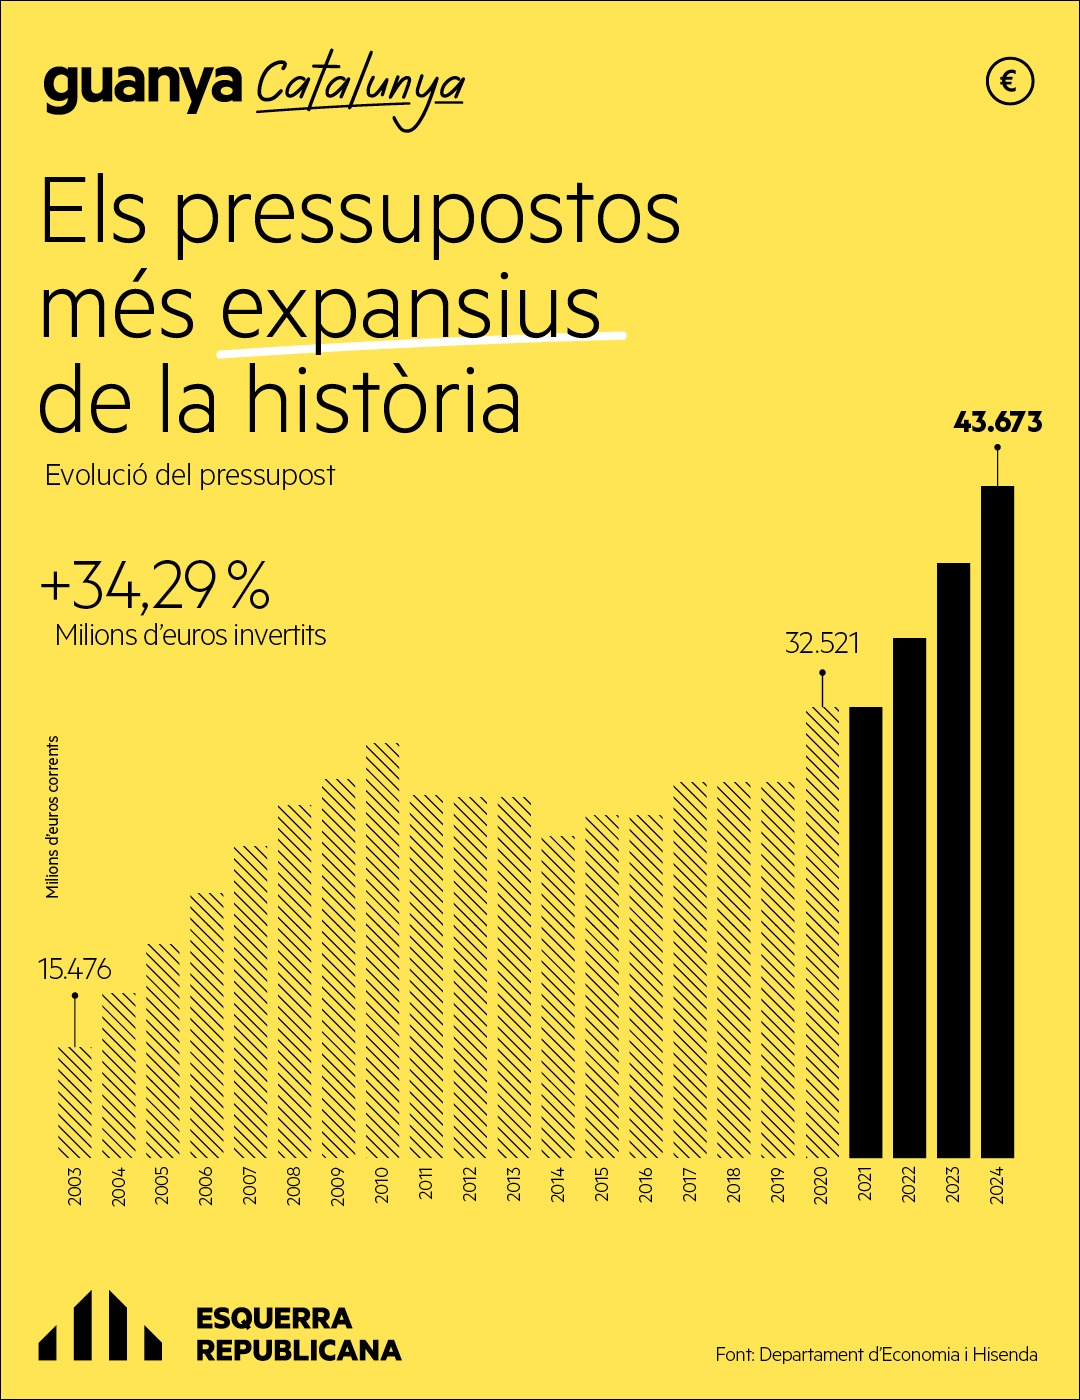
\includegraphics[width=0.55\linewidth]{misleading-chart.png}}
    \caption{Gràfic publicat per @Esquerra\_ERC a X el 30 de març de 2024,
      comparant el pressupost inicial de la Generalitat de 2003 amb el de 2024.
      Font: \url{https://x.com/Esquerra_ERC/status/1767926450135384275/photo/1}}
  \label{fig:original}
\end{figure}

\subsection{Anàlisi crítica }
\subsubsection{Principis de Tufte}
\begin{itemize}
  \item \textbf{Distorsió / \textit{lie factor}:} l'efecte real de l'increment pressupostari
  (15.693\,M€ el 2003 a 43.673\,M€ el 2024) és de $\times 2{,}78$, mentre que l'alçada
  de la barra de 2024 és 6 vegades la de 2003. Això dona un \emph{lie factor}
  $\approx 6/2{,}78 \approx 2{,}16$, bastant per sobre del marge acceptable ($0{,}95$--$1{,}05$)
  que proposa Tufte per considerar un gràfic honest.
  \item \textbf{Ràtio Dades-Tinta:} El gràfic no mostra cap eix Y graduat, de manera que el
  lector no pot verificar si les barres són proporcionals als valors reals i ha de confiar
  cegament en la impressió visual. A més, el bloc de color de fons i l'etiqueta destacada
  "+34,29\%" no aporten informació nova: són èmfasi retòric que competeix amb les dades
  en lloc de servir-les, cosa que redueix el ratio dades-tinta.
  \item \textbf{Integritat gràfica:} el gràfic viola directament el principi de Tufte segons
  el qual la representació visual d'una quantitat ha de ser proporcional a la magnitud
  numèrica que representa. Aquí la impressió visual (salt de $\times 6$) no es correspon
  amb la xifra real ($\times 2{,}78$), generant una incoherència entre el que es llegeix
  i el que es veu.
\end{itemize}

\subsubsection{Lleis de la Gestalt}
\begin{itemize}
  \item \textbf{Proximitat i continuïtat:} En mostrar només dues barres (2003 i 2024) en
  lloc de la sèrie completa, l'ull les interpreta com un salt directe "abans $\rightarrow$
  després", com si fossin dos passos consecutius d'una mateixa tendència. Això esborra
  visualment les dues dècades intermèdies i n'amaga l'evolució real, incloent-hi els anys
  sense pressupost aprovat.
  \item \textbf{Similitud:} les dues barres comparteixen exactament el mateix color i estil,
  cosa que fa que el cervell assumeixi automàticament que són comparables en igualtat de
  condicions, és a dir, que l'única diferència rellevant és l'alçada i que aquesta reflecteix
  fidelment la diferència real entre les dades.
  \item \textbf{Regió comuna:} el bloc de fons de color engloba tot el gràfic
  en una única unitat visual tancada, separada de la resta de la pàgina. Això fa que es
  percebi com un fet ja tancat i verificat, sense invitar el lector a qüestionar l'escala
  o a buscar-hi més context.
\end{itemize}

% =========================================================
\section{Modelitzacio de dades}

\subsection{El dataset}
El gràfic original només mostra tres punts (2003, 2020 i 2024): S'ha reconstruit tota la sèrie intermèdia. Ja que no
existeix cap CSV net amb aquestes dades, s’han combinat dues fonts:
\begin{itemize}
  \item \textbf{Portal de la Generalitat de Catalunya (2010–2023):} Com a font primària s’ha fet servir el dataset obert “Pressupostos aprovats de la
Generalitat de Catalunya”, consultat via la seva API SODA amb una query agregada per any. S’ha triat aquesta font per sobre d’altres perquè ve directament de l’organisme que elabora el pressupost, es
consulta amb una URL reproduïble i documenta explícitament el seu propi criteri de qualitat.

  \item \textbf{Institut d'Estadística de Catalunya (Idescat) (2003–2009):} Per als anys 2003–2009, el dataset anterior no arriba, i Idescat és l’única font pública disponible per a
aquest tram. S’ha usat com a font secundària, però ja que no ofereix una API ni una descàrrega neta per a aquesta sèrie, els valors s’han copiat a mà
llegint la seva pàgina. En contrastar anys solapats amb la font primària s'ha detectat una desviació
de fins al 30\%. El grau de confiança es consequentment menor.
\end{itemize}

Els anys amb pressupost prorrogat no disposen de dades, de manera
que l’absència d’un any hi és, per definició de l’organisme, l’evidència que aquell any no va tenir
pressupost nou.

Aquesta comprovació sobre la font primària també va revelar que 2024 tampoc no va tenir
pressupost nou aprovat: no apareix al dataset oficial, i ho confirma un document parlamentari
titulat “Pressupost per a l’exercici del 2024 (pròrroga)”. Els 43.673 M€ que fa servir el gràfic d’ERC
per a “2024” són només el projecte de pressupost que va aprovar el Govern en gabinet, que mai va
arribar a aprovar el Parlament per la convocatòria d’eleccions anticipades. Per això aquest treball fa
servir 41.024,72 M€, el pressupost de 2023, prorrogat com a valor real de 2024.

\subsection{Tecniques de preprocessament}
Codi complet a \texttt{src/build\_dataset.py}.
\begin{itemize}
  \item \textbf{Tractament dels anys sense pressupost nou aprovat}: Quan no s’aprova una llei de
pressupostos, el pressupost vigent es prorroga automàticament (no és un buit ni un zero, i tampoc
no és el projecte de llei no aprovat). S’ha arrossegat el valor nominal del darrer any efectivament
aprovat fins al següent any amb pressupost nou, i s’ha etiquetat cada any com a “aprovat” o
“prorrogat” per poder-los distingir visualment al redisseny.
  \item \textbf{Deflactació per IPC (euros constants de 2003)}: S’ha construït un índex IPC acumulat
any a any (base 2003 = 100) a partir de les variacions interanuals de l’INE, i s’ha dividit cada
valor nominal per aquest índex per obtenir el pressupost en poder adquisitiu constant. Sense
deflactar, part del creixement de les barres és pura inflació, no més despesa real.
  \item \textbf{Traçabilitat de la font per punt de dada}: Cada valor de la sèrie porta etiquetada la seva
font (API oficial / Idescat no verificat) i si prové d’un any amb pressupost nou o prorrogat, en
lloc de fondre-ho tot en una única sèrie homogènia aparentment fiable per igual d’un cap a l’altre.
\end{itemize}

\begin{table}[h!]
\centering \footnotesize
\begin{tabular}{lccrrr}
\toprule
Any & Pressupost nou & Font & Valor nominal (M€) & IPC (2003=100) & Valor processat (M€) \\
\midrule
2003 & sí & Idescat & 16.081,39 & 100,00 & 16.081,39 \\
2009 & sí & Idescat & 29.730,76 & 117,06 & 25.398,67 \\
2010 & sí & API oficial & 30.724,18 & 120,57 & 25.482,85 \\
2012 & sí & API oficial & 28.052,78 & 127,04 & 22.081,48 \\
2013 & \emph{no} & API oficial & 28.052,78 & 127,42 & 22.015,43 \\
2017 & sí & API oficial & 28.835,11 & 129,58 & 22.253,23 \\
2020 & sí & API oficial & 32.521,34 & 131,52 & 24.727,24 \\
2023 & sí & API oficial & 41.024,72 & 152,64 & 26.876,31 \\
2024 & \emph{no} & API oficial & 41.024,72 & 156,92 & 26.144,27 \\
\bottomrule
\end{tabular}
\caption{Extracte de la taula de dades reconstruïda. La sèrie completa (22 anys) es troba a \texttt{src/pressupost\_generalitat\_2003\_2024.csv}.}
\end{table}

% =========================================================
\section{Explicacio del redisseny}

\subsection{Eleccio del tipus de grafic}
Les dades són una sèrie temporal contínua (un valor per any, 22 anys). Per
Tufte, això demana un gràfic de línies, no barres. Les barres comuniquen comparacions puntuals
entre poques categories; una línia deixa veure la trajectòria, que és precisament el que el gràfic original
amagava en reduir-la a tres punts. S’ha apliquat que:
\begin{itemize}
  \item L'eix Y començi a zero
  \item Eixos etiquetats amb unitats (M€, anys), 
  \item Llegenda completa
\end{itemize}
S'ha afegit també una codificació visual que distingeix els anys amb pressupost nou aprovat
(cercle ple) dels anys prorrogats (cercle buit), una informació que el gràfic d’ERC ometia

\begin{figure}[h!]
  \centering
  \fbox{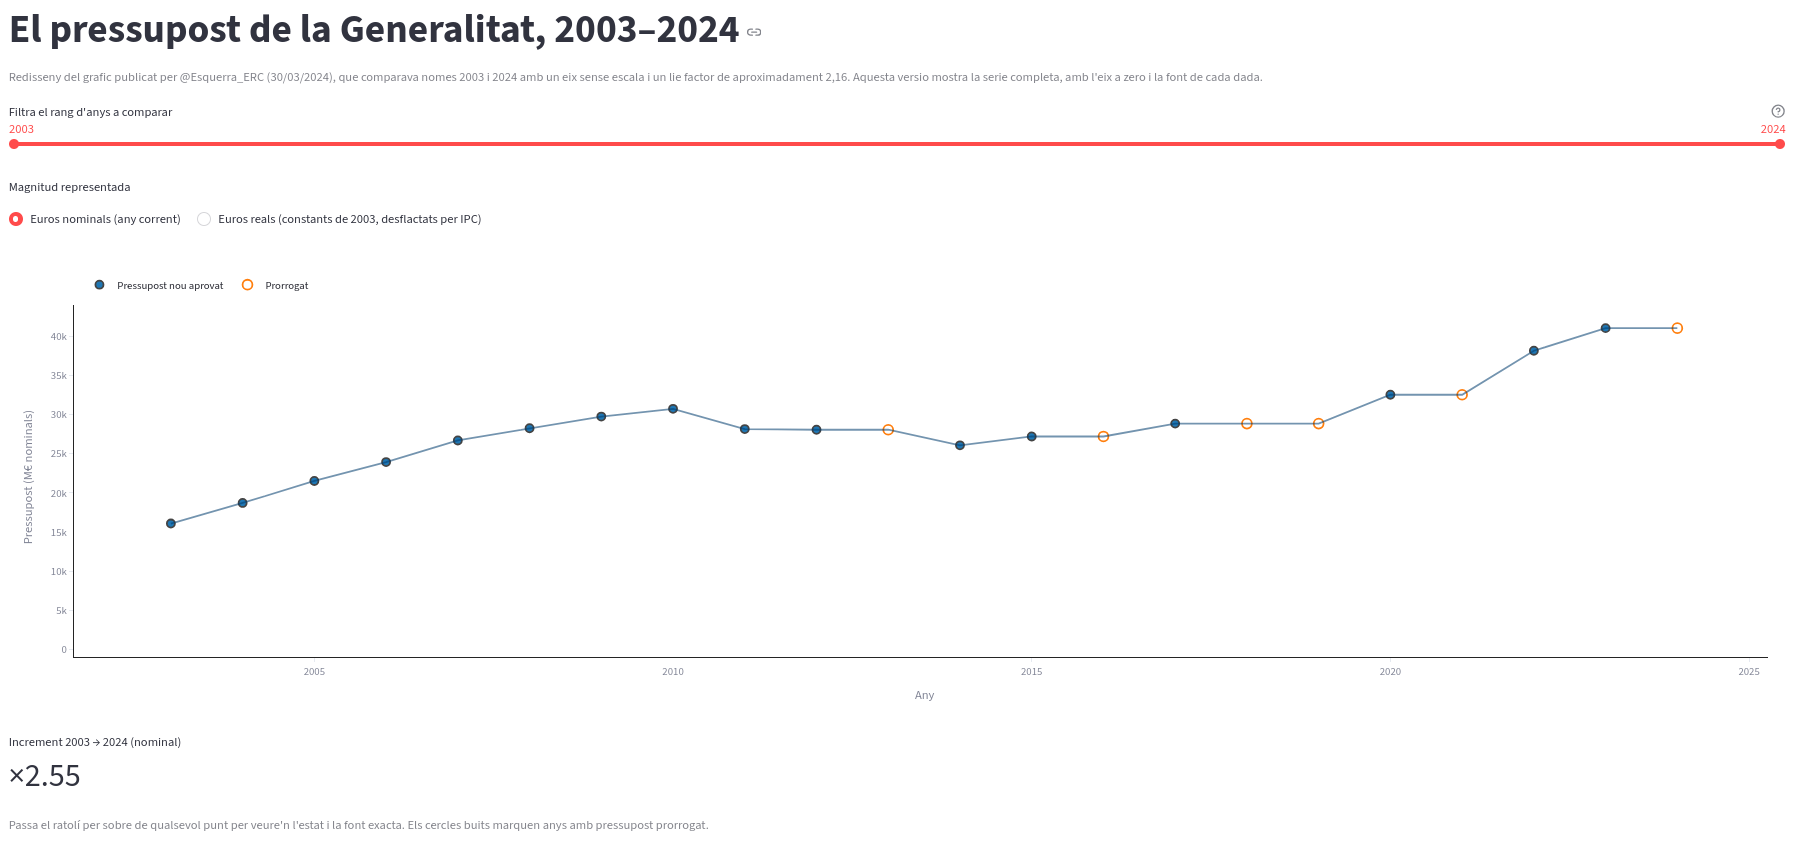
\includegraphics[width=0.9\linewidth]{modified-chart.png}}
  \caption{Redisseny: aplicació Streamlit + Plotly (\texttt{src/02\_app\_redisseny.py}), amb la magnitud commutada
a euros reals (constants de 2003) i el rang complet 2003–2024 seleccionat.}
  \label{fig:redisseny}
\end{figure}

\subsection{Interactivitat implementada}
S’han implementat tres tipologies:
\begin{itemize}
  \item \textbf{Abstraure/Elaborar:} En passar el ratolí per sobre de qualsevol punt apareix l’any,
l’estat (aprovat/prorrogat), la font exacta de la dada, i els valors nominal i real (Figura 3). Millora
la usabilitat perquè dona feedback immediat sense sobrecarregar el gràfic base.
  \item \textbf{Codificar:} Un selector canvia en viu la magnitud representada entre euros
nominals i euros constants de 2003. Deixa que sigui el propi usuari qui comprova que bona part del çreixement del
pressupost és inflació i no despesa real.
\item \textbf{Filtrar:} Un control de rang permet acotar la comparació a qualsevol parell d’anys,
inclosos exactament 2003 i 2024. La mètrica sota el gràfic es recalcula automàticament
per al rang triat
\end{itemize}

\begin{figure}[h!]
  \centering
  \fbox{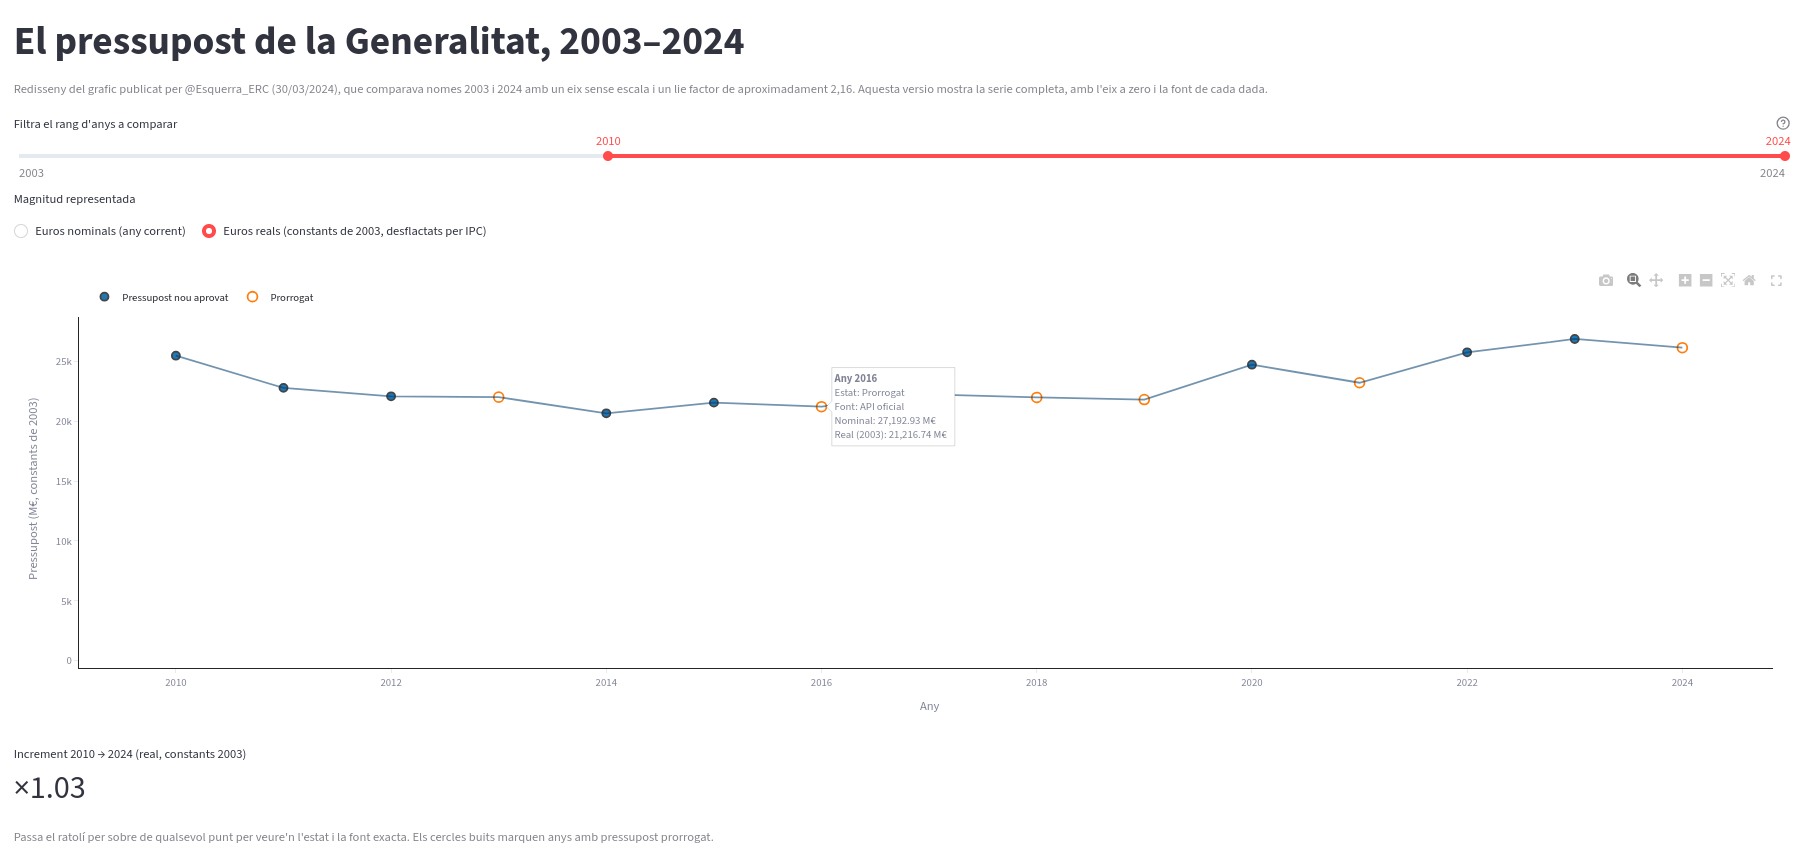
\includegraphics[width=0.9\linewidth]{modified-chart_1.png}}
  \caption{Les tres tipologies d'interacció a la vegada: \textbf{Filtrar} (rang acotat a
2010–2024), \textbf{Codificar} (magnitud commutada a euros reals, constants de 2003) i
\textbf{Abstraure/Elaborar} (\emph{tooltip} sobre l'any 2016, que mostra el seu estat prorrogat, la font i els valors nominal i real). La mètrica inferior es recalcula en
viu per al rang seleccionat: $\times$1,03 en euros reals entre 2010 i 2024.}
\end{figure}

% =========================================================
\section{Annex tècnic}

\textbf{Repositori de codi:} \url{https://github.com/khadyyade/miv-practica1}

\textbf{Eines emprades:} Python 3 (\texttt{pandas} per a la reconstrucció i deflactació
de la sèrie, \texttt{urllib}/\texttt{json} per a la crida a l'API oberta), Plotly
(\texttt{graph\_objects}) per al gràfic interactiu, i Streamlit per als controls i
l'aplicació web.

\textbf{Estructura del repositori:}
\begin{itemize}\footnotesize
  \item \texttt{main.tex} --- aquest informe.
  \item \texttt{src/01\_build\_dataset.py} --- reconstrucció de la sèrie: crida a l'API
  oberta (font primària, 2010--2023), dades manuals d'Idescat (font secundària, 2003--2009),
  tractament de la pròrroga i deflactació per IPC. Genera
  \texttt{src/pressupost\_generalitat\_2003\_2024.csv}.
  \item \texttt{src/pressupost\_generalitat\_2003\_2024.csv} --- sèrie reconstruïda, amb
  font i estat (aprovat/prorrogat) per a cada any.
  \item \texttt{src/02\_app\_redisseny.py} --- aplicació Streamlit + Plotly del redisseny
  interactiu (Secció 3).
  \item \texttt{src/requirements.txt} --- dependències de Python.
  \item \texttt{img/} --- captures utilitzades en aquest informe.
\end{itemize}

\textbf{Per reproduir-ho:}
\begin{enumerate}\footnotesize
  \item \texttt{pip install -r src/requirements.txt}
  \item \texttt{python3 src/01\_build\_dataset.py} --- descarrega les dades en directe de
  l'API i regenera el CSV (cal connexió a internet).
  \item \texttt{streamlit run src/02\_app\_redisseny.py} --- obre l'aplicació interactiva
  al navegador.
\end{enumerate}

\end{document}